\documentclass{report}  % Tipo de documento (puedes cambiarlo a report, book, etc.)
\usepackage[utf8]{inputenc}  % Codificación de caracteres (importante para acentos y ñ)
\usepackage[backend=biber]{biblatex}
\usepackage[scaled=1.05,proportional,lightcondensed]{zlmtt}
\renewcommand*\familydefault{\ttdefault} %% Only if the base font of the document is to be typewriter style
\usepackage[T1]{fontenc}
\usepackage[table]{xcolor}
\addbibresource{bibliografia.bib}

\renewcommand{\thechapter}{\arabic{chapter}} % Si usas \chapter
\renewcommand{\thesection}{\arabic{section}}
\renewcommand{\thesubsection}{\thesection.\arabic{subsection}}
\renewcommand{\thesubsubsection}{\thesubsection.\arabic{subsubsection}}
\renewcommand{\theparagraph}{\thesubsubsection.\arabic{paragraph}}


\usepackage{graphicx}        % Para incluir imágenes
\usepackage{caption}         % Para configurar las leyendas de las figuras y tablas
\usepackage{amsmath}         % Paquetes matemáticos
\usepackage{geometry}        % Configurar márgenes
\usepackage{titling}        % Configurar el título
\geometry{a4paper, margin=1in}

\title{PulpaSA}  % Título del documento
\author{Jesús Romeo Mougán}                     % Autor
\date{\today}                           % Fecha (puedes poner una fija o usar \today)

\begin{document}

\captionsetup{aboveskip=5pt, belowskip=10pt}

\begin{titlepage}
    \newgeometry{top=3cm, bottom=3cm} % Modifica márgenes de la portada
    \centering
    \vspace*{\fill} % Empuja el contenido hacia el centro

    %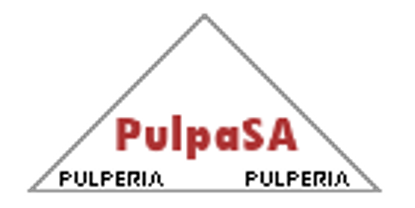
\includegraphics[width=0.5\textwidth]{images/image.png} 
    %\vspace{2cm}

    {\Huge \textbf{\thetitle}} \\[1cm]
    {\large Game Design Document} \\[1.5cm]

    \vspace*{\fill}

    {\large \textbf{\theauthor}} \\ [1cm]
    {\large IES San Clemente} \\[4cm]

    \vspace*{\fill} % Empuja hacia la parte inferior

    {\large \today}

    \restoregeometry % Restaura los márgenes normales para el resto del documento
\end{titlepage}



\renewcommand{\contentsname}{Índice}

\tableofcontents

% start sections by 1

\newpage

\section{Mecánicas}
\definecolor{octopus}{HTML}{CE2093}

\begin{table}[h]
    \centering
    \renewcommand{\arraystretch}{1.3} % Aumenta la altura de las filas
    \setlength{\tabcolsep}{10pt} % Espaciado entre columnas
    \label{tab:mecanicas}
    \rowcolors{2}{gray!15}{white} % Colores alternos en las filas
    \begin{tabular}{|p{4cm}|p{2cm}|p{3cm}|p{4cm}|}
        \hline
        \rowcolor{octopus} % Color de fondo para la fila del encabezado
        \textbf{Mecánica}  & \textbf{Tipo} & \textbf{Necesidad} & \textbf{Reglas} \\
        \hline
        Atender Comandas & Primaria  & Interaccion con obxectos  & Os xogadores deben xestionar pedidos de clientes \\
        \hline
        Coordinación cooperativa & Primaria  & Multixogador    & Se permite atacar enemigos con un arma o golpe cuerpo a cuerpo. \\
        \hline
        Preparación de ingredientes  & Secundaria & Interacción con obxectos & Cortar cachelos/polbo antes de cocelos \\
        \hline
        Cocción & Secundaria & Xestión do transcurso do tempo / FSM & Estar pendente da cocción dos ingredientes \\
        \hline
        Condimentación & Secundaria & Interacción con obxectos & Engadir sal, pementa, aceite, etc. \\
        \hline
        Limpeza de pratos & Secundaria & Interacción con obxectos & Limpar cando se esgoten \\
        \hline

    \end{tabular}
    %\caption{Táboa de Mecánicas}
\end{table}


\section{Narrativa}

Pese a que PulpaSA é un xogo plenamente de xestión, tentarase darlle un contexto histórico sinxelo con un toque humorístico.

\subsection{Idea}

Videoxogo de xestión cooperativa dunha pulpería ambulante, onde cada nivel correspondería a unha romería galega.

\subsection{Logline}

Os xogadores traballan nunha pulpería ambulante durante unha romaría galega, onde deben coordinarse para servir pratos de polbo baixo presión.

\subsection{Sipnose}

Un grupo de amigos norteamericanos, que orixinariamente traballaban arreo nunha consultoría de software, e eran víctimas do burnout, deciden
abandonar todo e montar unha pulpería coa que percorrerán toda a xeografía galega en busca de romarías onde poidan ir acadando boa fama.
 Todo isto ocorre despois de que o grupo viñese de vacacións a Galicia, e quedasen ledos coa cultura
e tradición. A idea de montar unha pulpería ambulante xurdiu nunha noite de copas, e aínda que ao principio parecía unha idea disparatada,
acabou por materializarse. O inicio non será fácil... pero coa tua axuda, poderán conseguilo!

\subsection{Arquetipo}

PulpaSA toma como referencia o arquetipo do heroe:
%listar arquetipos
\begin{itemize}
    \item \textbf{O heroe}: Os protagonistas deciden abrir a pulpería
    \item \textbf{Desafíos iniciais}: Aprender a xestionar a pulpería
    \item \textbf{Complicacións}: Incrementase cada vez máis a demanda / complexidade dos pedidos
    \item \textbf{Clímax}: A pulpería logra acadar os obxectivos mínimos
    \item \textbf{Resolución}: PulpaSA é un éxito
\end{itemize}

\subsection{Estrutura Narrativa}

O xogo, en canto a estrutura narrativa, dividirase en 3 seccións claramente diferenciadas (introducción, nudo e desenlace):

\begin{itemize}
    \item \textbf{Inicio}: Introdución ao xogo, pequena animación onde se presenta o contexto do xogo e se ensinan as mecánicas clave.
    \item \textbf{Nudo}: Cada un dos niveis que o xogador terá que superar
    \item \textbf{Desenlace}: Animación final onde se caricaturiza o éxito (ou quizáis o fracaso) da pulpería
\end{itemize}

\subsection{Elementos adicionais}

\subsubsection{}

\section{Personaxes}
O xogo, nun escenario ideal, contaría con 4 personaxes xogables a elexir,

\subsection{Personaxe 1}
\subsubsection{Nombre}
John Cea
\subsubsection{Importancia en el Juego}
Socio fundador de PulpaSA
\subsubsection{Rasgos característicos}
Ten a capacidade de limpar os pratos máis rápido
\subsubsection{Transformación}

\subsection{Personaxe 2}
\subsubsection{Nombre}
Bill Portas
\subsubsection{Importancia en el Juego}
Socio fundador de PulpaSA
\subsubsection{Rasgos característicos}
Ten a capacidade de cortar os ingredientes máis rápido
\subsubsection{Transformación}
Os personaxes non teñen unha transformación, dado que é un xogo de xestión, onde prima a habilidade e rapidez dos xogadores.


\subsection{Personaxe 3}
\subsubsection{Nombre}
Ariana Pequena
\subsubsection{Importancia en el Juego}
Socio fundador de PulpaSA

\subsubsection{Rasgos característicos}
Ten a capacidade de cocer os ingredientes máis rápido
\subsubsection{Transformación}
Os personaxes non teñen unha transformación, dado que é un xogo de xestión, onde prima a habilidade e rapidez dos xogadores.


\subsection{Personaxe 4}
\subsubsection{Nombre}
Natalie Newport
\subsubsection{Importancia en el Juego}
Socio fundador de PulpaSA
\subsubsection{Rasgos característicos}
Ten a capacidade de condimentar con 2 condimentos na mesma acción
\subsubsection{Transformación}
Os personaxes non teñen unha transformación, dado que é un xogo de xestión, onde prima a habilidade e rapidez dos xogadores.

\end{document}
